\documentclass[12pt,letterpaper,answers]{exam}
%\usepackage{color}
\usepackage[usenames,dvipsnames,svgnames,table]{xcolor}
\usepackage[margin=0.9in]{geometry}
\renewcommand{\familydefault}{\sfdefault}
\usepackage{multicol}
\pagestyle{head}
\definecolor{c03}{HTML}{FFDDDD}
\header{AM 108 Problem Set 08}{}{{\colorbox{c03}{\makebox[3.0cm][l]{Due Fri Mar 31}}}\\ at noon}
\runningheadrule
\headrule
\usepackage{diagbox}
\usepackage{graphicx} % more modern
%\usepackage{subfigure} 
\usepackage{amsmath} 
\usepackage{amssymb} 
%\usepackage{gensymb} 
%\usepackage{natbib}
\usepackage{hyperref}
%\usepackage{enumitem}
%\setlength{\parindent}{0pt}
%\usepackage{setspace}
%\pagestyle{empty}  
%\newcommand{\Sc}[0]{
%{\color{BlueViolet}\S}
%}
\usepackage{tcolorbox}
\usepackage[framed,numbered,autolinebreaks,useliterate]{mcode}

\begin{document}
 \pdfpageheight 11in 
  \pdfpagewidth 8.5in


\noindent\textbf{Problem Set Instructions:}  
\begin{itemize}
\itemsep0pt
\item In your first attempt of the problem set problems, you are encouraged to treat the problem set as an open-notes quiz.  Work on it without consulting classmates, Ed, course staff, other people, other internet resources, or any solutions or answers.  Work on each problem, completing as much as you are able to, and making a note in your work whenever you become stuck or confused.
\item After your initial individual attempt, collaboration is encouraged (see guidelines below) as you continue to work on the problems.  You'll submit a pdf of this work as part of your problem set submission on Gradescope (and will also submit it on Canvas).
\item Submit the pdf of your problem set work with the problems written up in order (computational work should be included: it can be at the end of the pdf) on Canvas and access the solutions.
\item Complete the reflection questions below, and submit that reflection work, along with your problem set pdf, on Gradescope.
\end{itemize}
  
\noindent\textbf{Submission Instructions:}  
\begin{itemize}
\item Following the instructions above, upload a pdf of your work to Canvas.  Upload your reflection answers and the pdf to Gradescope.
\item If you would like to use mathematical software other than Mathematica, that's fine. 
\end{itemize}

\noindent\textbf{Late Work Policy:}
\begin{itemize}
\itemsep0pt
\item Problem sets are accepted up to eight hours late with no penalty (8pm Friday). 
\item Three 36 hour late days are available to every student (three extensions to 8pm on Saturday).  These late days are expected to be used for unexpected illness or other conflicts.
\item Additional late days are not typically 
available.
\item Problem sets are not accepted beyond the late deadline.
\end{itemize}

\noindent\textbf{Collaborating on Problem Sets:}  

\noindent Collaborating with classmates in planning and designing solutions to homework problems is encouraged.  Collaboration, cooperation, and consultation can all be productive.  Work with others to: 
\begin{multicols}{2}
\begin{itemize}
\itemsep-0.2em
    \item discuss the problem
    \item brainstorm
    \item walk through possible strategies
    \item outline solution methods
\end{itemize}   
\end{multicols}

\noindent For homework, you may consult or use:
\begin{multicols}{2}
\begin{itemize}
\itemsep-0.2em
    \item Course text (including answers in back)
    \item Your notes (taken during class)
    \item Class notes of other students
    \item Course handouts
    \item Canvas posts/Ed posts
    \item Computational tools such as Python, Mathematica, or Desmos
    \item Calculators
    \item Other books
    \item the Internet
\end{itemize}
\end{multicols}

\noindent You may:
\begin{itemize}
    \item Look at communal work while writing up your own solution
\end{itemize}

\noindent You may \textbf{not}:
\begin{itemize}
\itemsep-0.2em
    \item Look at the individual work of others while writing up your own solutions
    \item Post about problems online
\end{itemize}


\noindent Do \textbf{not} consult the following resources until after you think you have solved a problem, have fully written up your answer, and have submitted a pdf of your work to Canvas.
%\begin{multicols}{2}
\begin{itemize}
\itemsep-0.2em
    \item The text solution manual
    \item The posted solutions
    \item Other solutions (from previous years, from sites like Chegg or Math Stackexchange, etc)
\end{itemize}
%\end{multicols}


%\eject


% \begin{enumerate}
% \item Reflection questions

\section*{Reflection questions}
Submit these on Gradescope.
\begin{enumerate}
\item \begin{enumerate}
    \itemsep0pt
    \item When you worked on the problems individually, how did each problem go?
    \item Where did you get stuck or confused?  For any subpart where you were stuck or confused be specific.  \emph{For example 'I tried to use the hint for 3b, but I couldn't find a way to relate $r$ and $x$'.}
    \item What additional progress were you able to make when you consulted other people or additional resources?
    \item For each part of each problem, how did your work compare with the posted solution?  Identify similarities and differences.
\end{enumerate}  
\item For any problems you were not able to complete, what made them difficult to complete?  What did you learn from the posted solution?
\item What aspects of the course challenged you this week?  What did you do to address those challenges?  What topics/ideas/procedures do you not yet understand?
\item What did you understand the best this week?  What, if anything, do you understand better this week than you did in the past?
\item List the people that you worked with or consulted on the problem set problems.  This might include other students in the course, course instructors, or people who have previously taken the course.
\item Below, indicate how much of your time for this class has been doing the following activities:
	\begin{enumerate}
	\item Working on problem set problems or other practice problems alone
	\item Viewing preclass materials or reviewing course materials, including problem set solutions, alone
	\item Working on problem sets, reviewing notes, or discussing course topics with your classmates
	\item Working through supplementary materials
	\item Going to office hours
    \item Working individually on the project
    \item Working with your team on the project
	\item Other (please specify)
	\end{enumerate}

\end{enumerate}



\begin{questions}

\question (variation on 8.2.6: Hopf bifurcation) 

Let $\dot x = \mu (x - 1) + y - (x-1)^3, \dot y = -(x-1) + \mu y - 2 y^3$.  A Hopf bifurcation occurs at $(1,0)$ for $\mu = 0$. 

On either side of the bifurcation: Provide phase portraits and add numerically approximated trajectories for the forwards time version of the system, and also for the backwards time version of the system.

Use your work to decide whether the bifurcation appears to be supercritical or subcritical.  

\emph{Identifying whether 8.2.5 appears to be subcritical or supercritical is worked as an example in the provided Mathematica/Python notebooks.}

\unframedsolutions

\begin{solution}

We are interested in the fixed point at $(1,0)$.  Jacobian: $\left(\begin{array}{c c} \mu -3(x-1)^2 & 1 \\ -1 & \mu - 6y^2\end{array}\right)$.  At $(0,0)$: $\left(\begin{array}{c c} \mu  & 1 \\ -1 & \mu \end{array}\right)$.  Trace is $2\mu$ and determinant is $\mu^2 + 1$.  Hopf bifurcation at $\mu = 0$.  Repeller for $\mu > 0$ and attractor for $\mu < 0$.

Using backwards time:

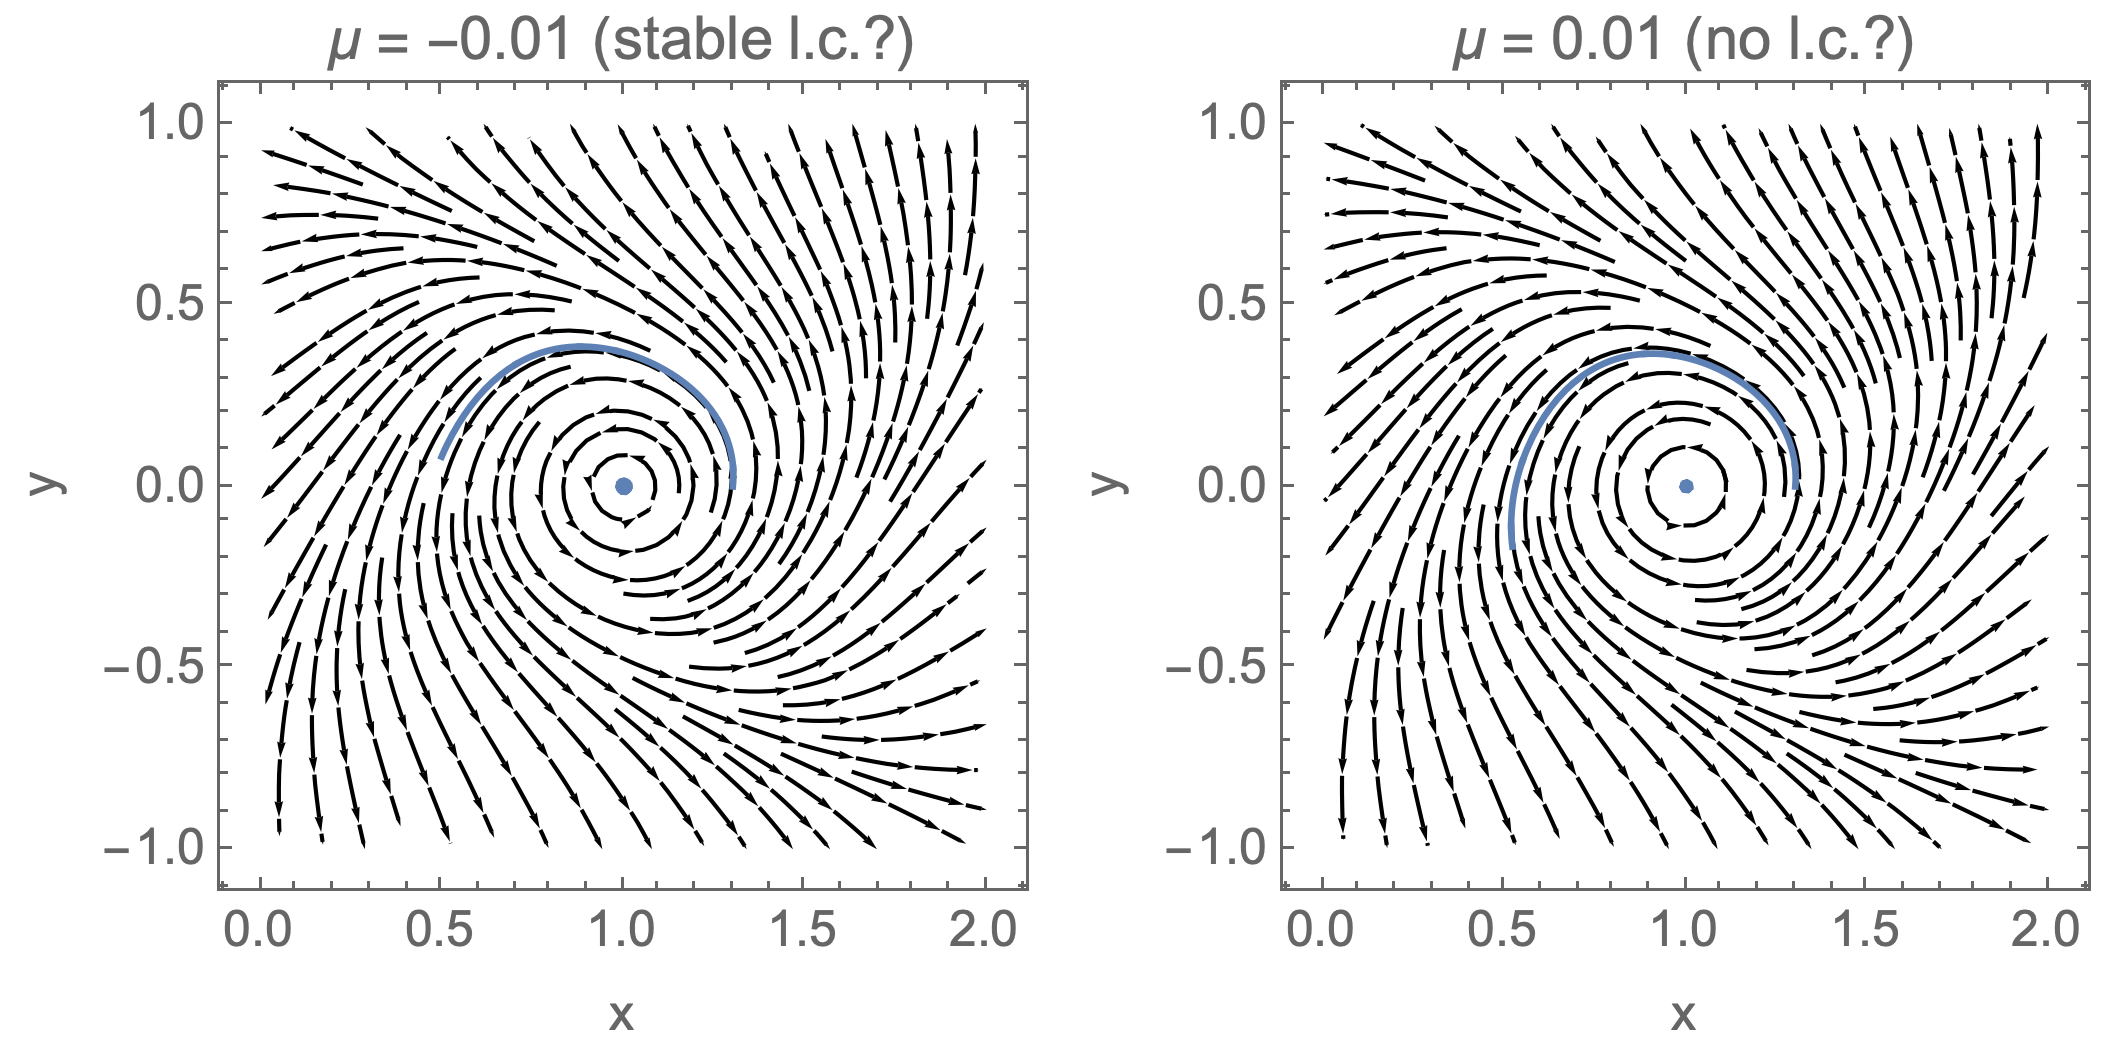
\includegraphics[width=\textwidth]{img/PS08-S23-q1.png}


Using forward time:

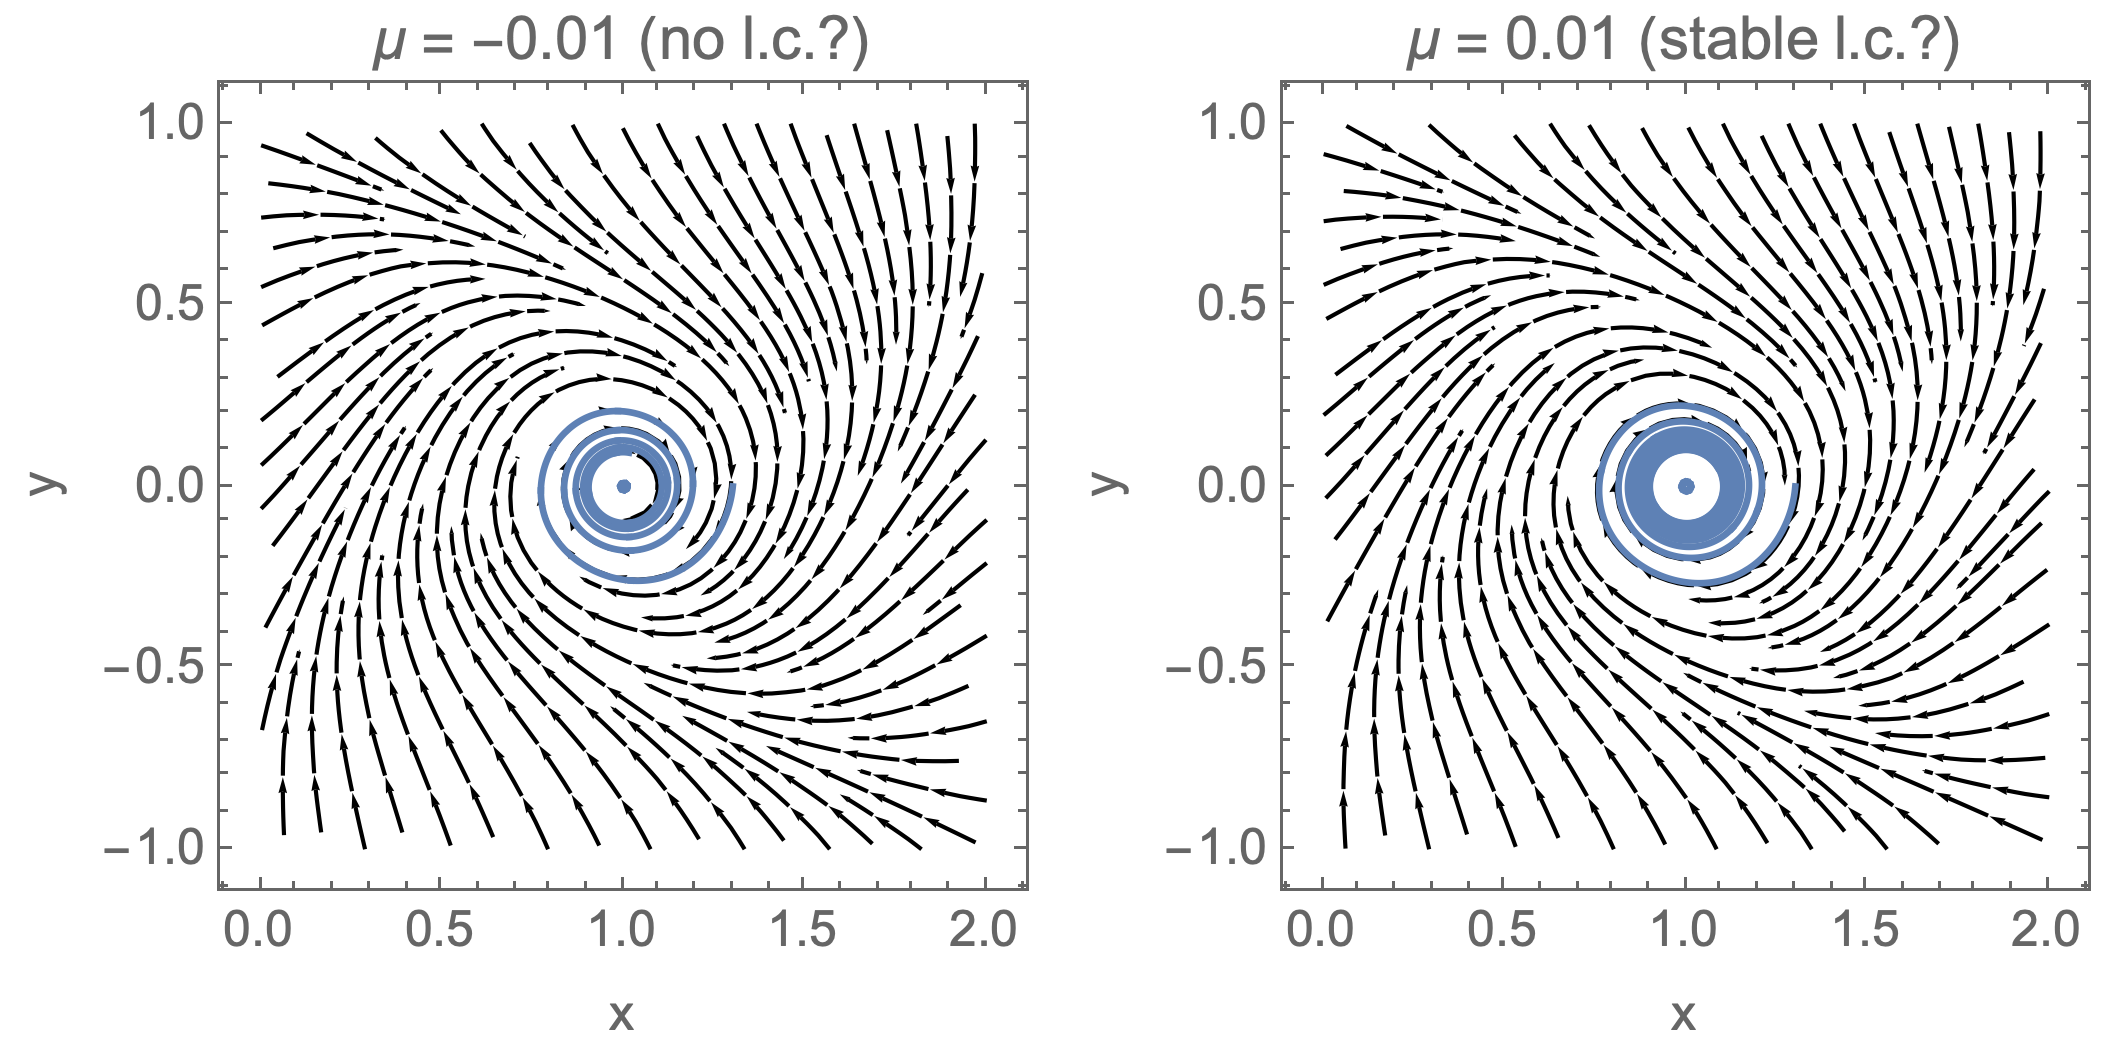
\includegraphics[width=\textwidth]{img/PS08-S23-q1c.png}

If the bifurcation is subcritical: in backwards time the fixed point switches stability.  It is a repeller for $\mu < 0$ and an attractor for $\mu > 0$.  If the limit cycle of the forward time system is unstable (subcritical Hopf) the limit cycle would be around the attractor of the forward system.  That means we are looking for a stable limit cycle in backwards time when $\mu < 0$ and a stable fixed point for $\mu > 0$.  Instead, we see repelling behavior in both phase portraits.  That means we are likely seeing repulsion from the fixed point for $\mu < 0$ and repulsion from a limit cycle for $\mu > 0$.

If the bifurcation is supercritical: no limit cycle for $\mu < 0$ and an attracting fixed point, so trajectories would approach the fixed point.  A stable limit cycle for $\mu > 0$ so trajectories would approach that.

This appears to be our situation.  Plotting trajectories vs time allows us to see the attracting behavior.

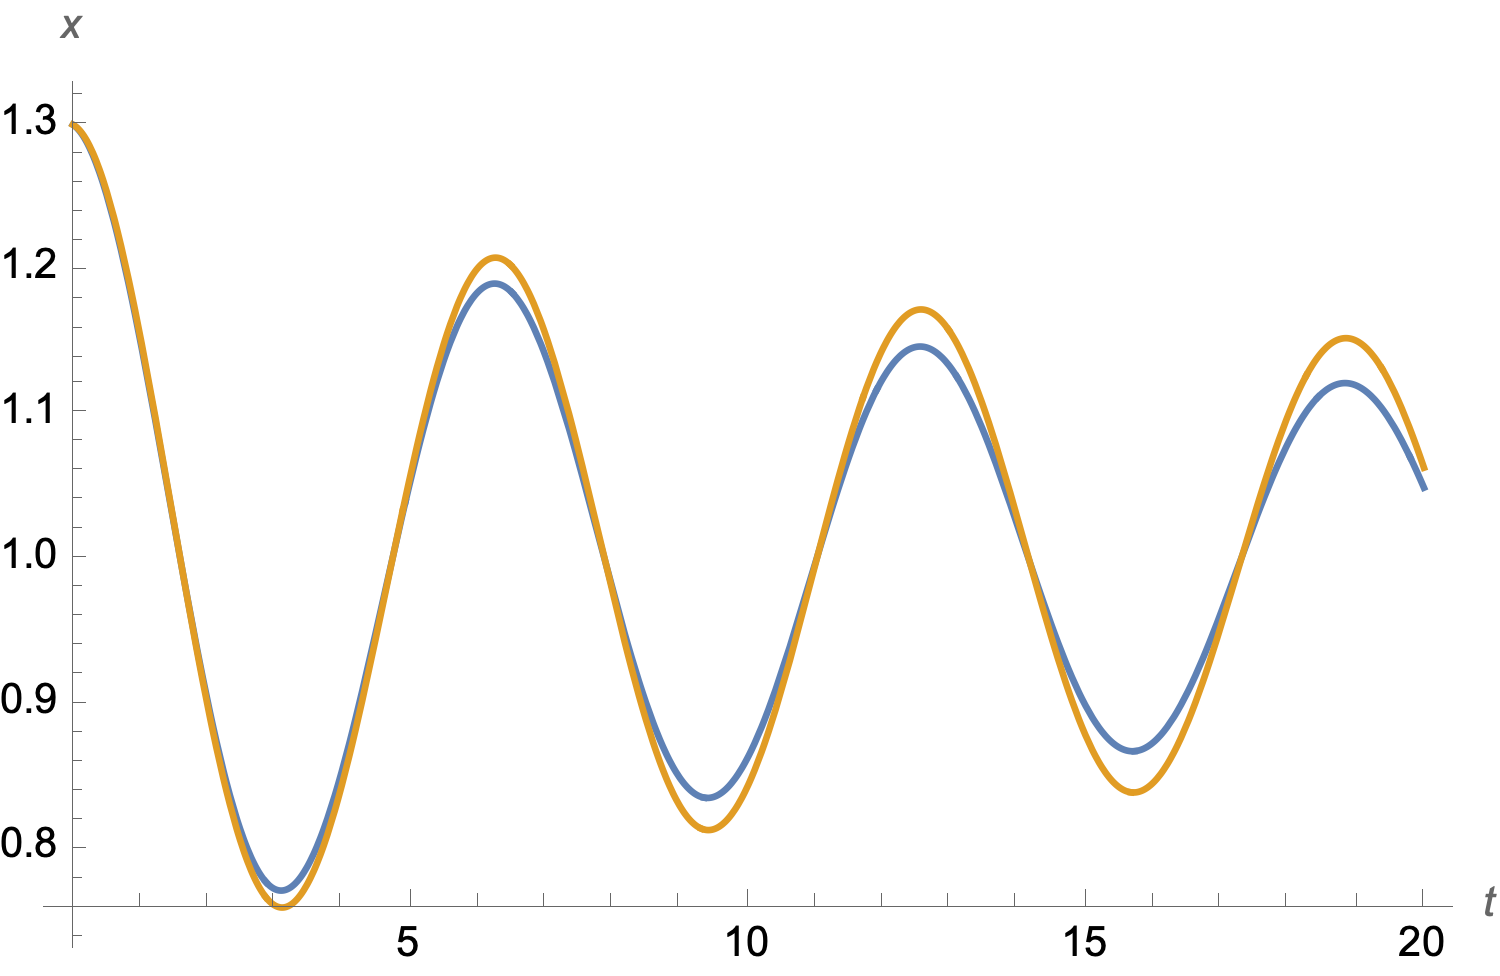
\includegraphics{img/PS08-S23-q1d.png}

It appears to be a supercritical Hopf.
\end{solution}


\question (Poincar\'e map).  

Use the forward time system for this problem.
\begin{parts}
    \item For the system above, create a Poincar\'e map for $\mu = 0.01$ and $\mu = -0.01$.  Determine whether there is a closed orbit for $\mu > 0$ or for $\mu < 0$, use the map to identify the stability of the orbit, and provide an estimate of the amplitude of the orbit.
    \item If there is a closed orbit for $\mu>0$, create a Poincar\'e map for $\mu = 0.05$.  Provide an estimate of the amplitude of the orbit.  If there is a closed orbit for $\mu<0$, do this work for $\mu = -0.05$ instead.
\end{parts}

\emph{There is a Mathematica/Python Poincar\'e map example in the notebooks.  We are approximating the map (at a few values of the domain) numerically, rather than exactly finding the map analytically.}

\begin{solution}

The Hopf appears to be supercritical so use $\mu = 0.01$ and $\mu = 0.05$.

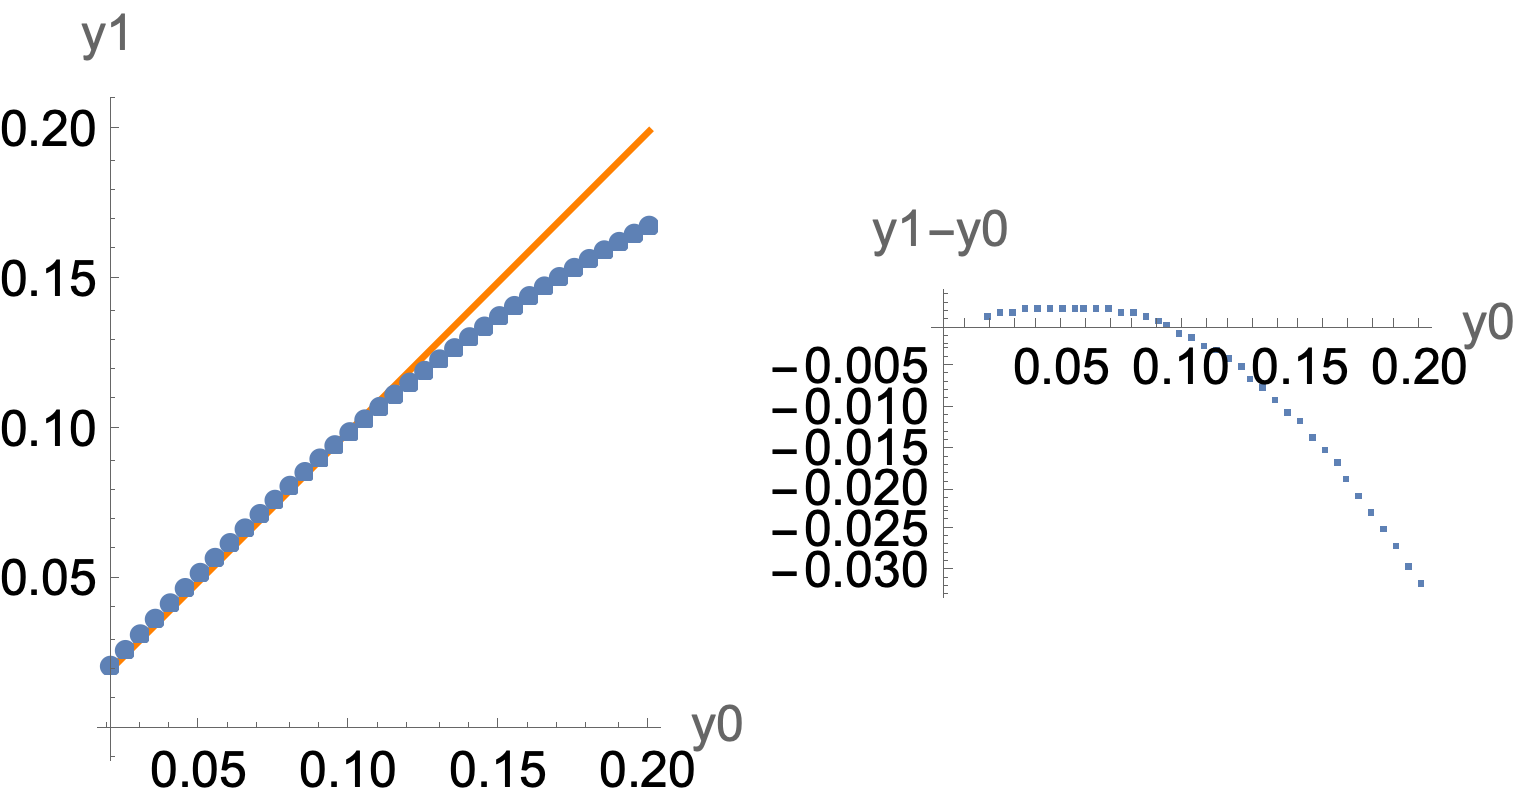
\includegraphics{img/PS08S23poincaremap1.png}

For $\mu = 0.01$ the limit cycle is at about $0.1$ in amplitude (radius) and is stable based on the slope.

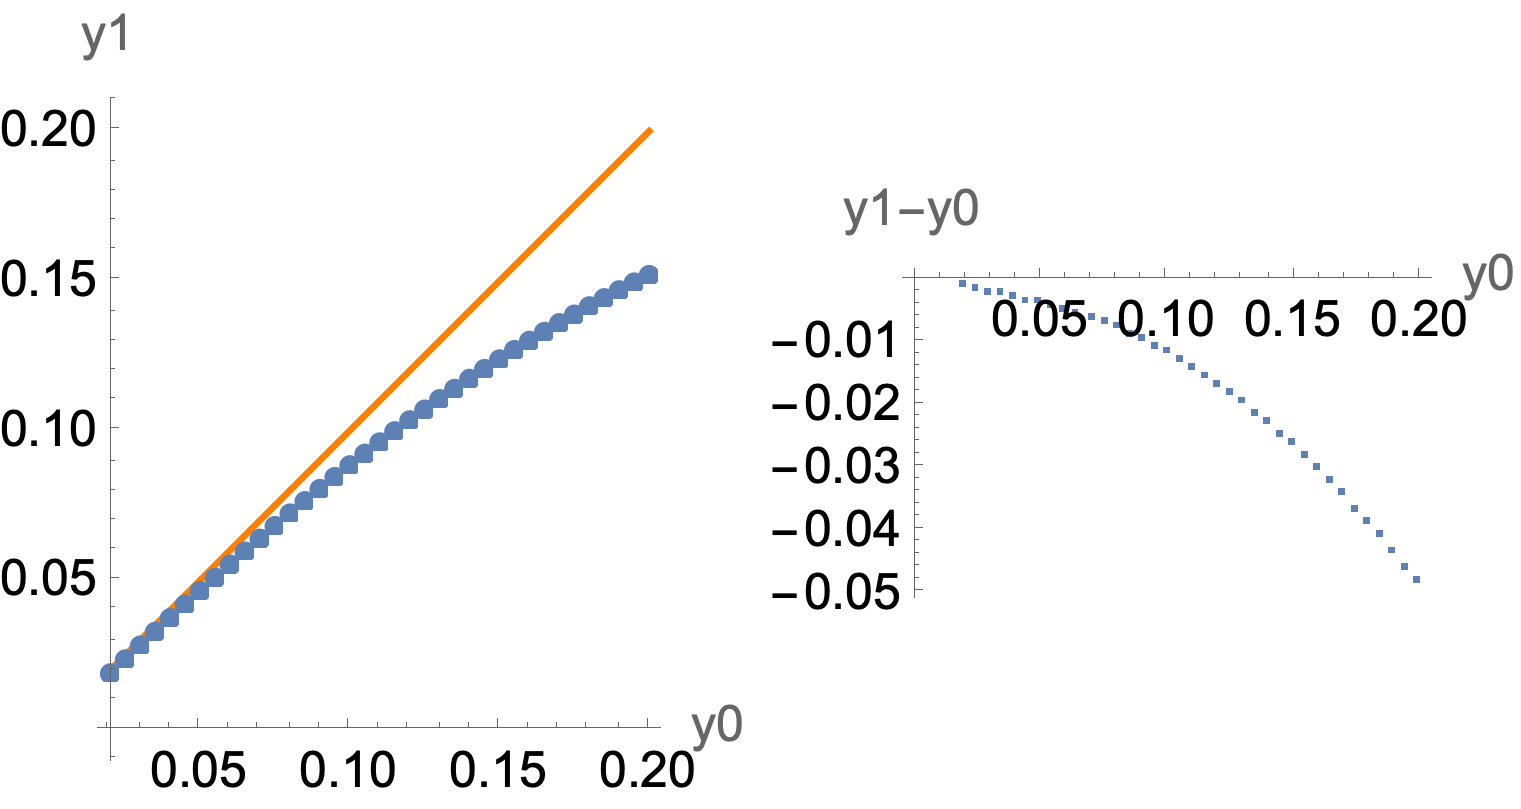
\includegraphics{img/PS08S23poincaremap-1.png}

For $\mu = -0.01$ there is not a limit cycle (no fixed point of the map away from zero).

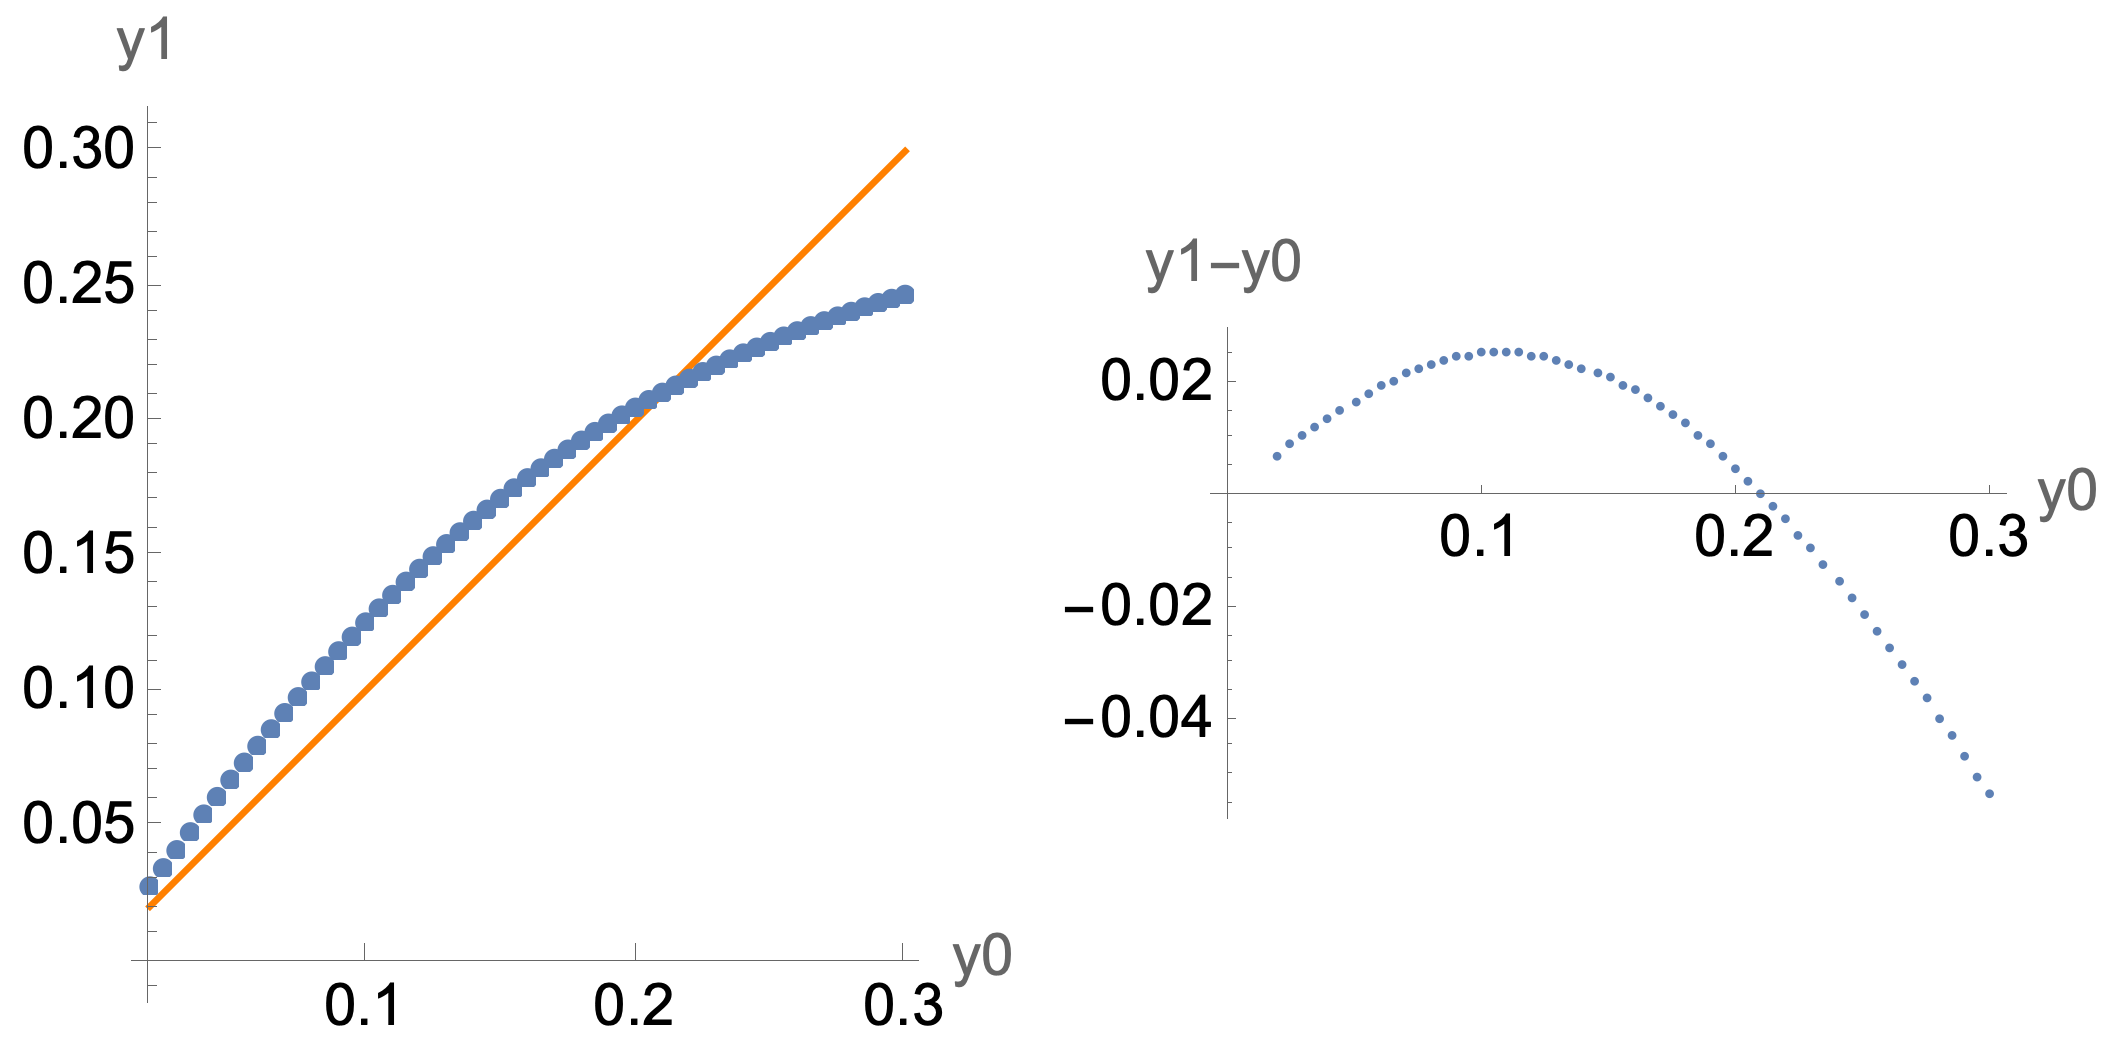
\includegraphics[width=\textwidth]{img/PS08S23poincaremap5.png}

For $\mu = 0.05$ the limit cycle is at about $0.21$ in amplitude (radius) and is stable based on the slope.

\end{solution}

\question (8.3.1) Brusselator model of a chemical oscillator
\begin{parts}
\item Do part (a) as written.  \emph{You can use Mathematica/Python or do this by hand}.
\begin{solution}
Find the fixed points: $\dot y = x(b-axy)$ so $x=0$ or $xy = b/a$ at fixed points.

$\dot x = 1-(b+1)x + ax^2y$.  When $x = 0$, $\dot x = 1$ so there is no fixed point.  When $xy = b/a$, $1-(b+1)x + ax(b/a) = 0 \Rightarrow 1 -(b+1)x + b x = 0$.  $\Rightarrow x = 1$ at the fixed point.  There is one fixed point at $(1, b/a)$.

Classifying: the Jacobian is $\left(\begin{array}{c c} 
-(b+1) + 2axy & ax^2 \\
b - 2axy & -ax^2\end{array}\right)$.

At the fixed point, this is $\left(\begin{array}{c c} 
b-1 & a \\
-b & -a\end{array}\right)$.

Trace is $-a + b - 1$ and determinant is $(b-1)(-a)+ab = -ab + a + ab = a$.  For $a>0$ this is a repeller or attractor, as set by the trace.  When $b<a+1$ we have an attractor.  When $b>a+1$ we have a repeller (Hopf bifurcation at $b_c = a+1$).
\end{solution}
\item Sketch the nullclines for $a=1,b=3$, and provide representative vectors in the four different sectors.  Sketch a plausible trapping region.  \emph{You do not need to rigorously show that it is actually a trapping region, but do choose it so that no vectors are obviously pointing outwards}.
\begin{solution}

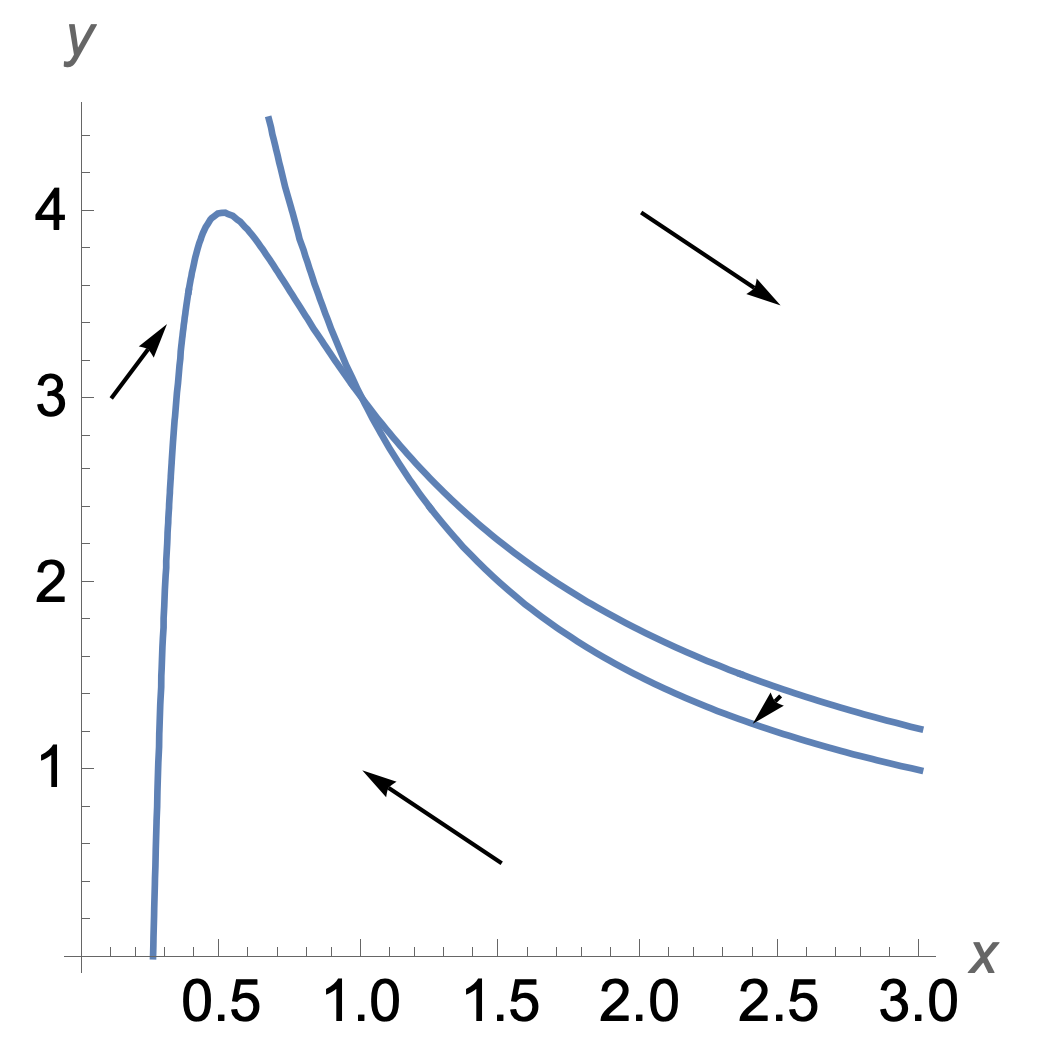
\includegraphics{img/PS08S23brusselator.png}

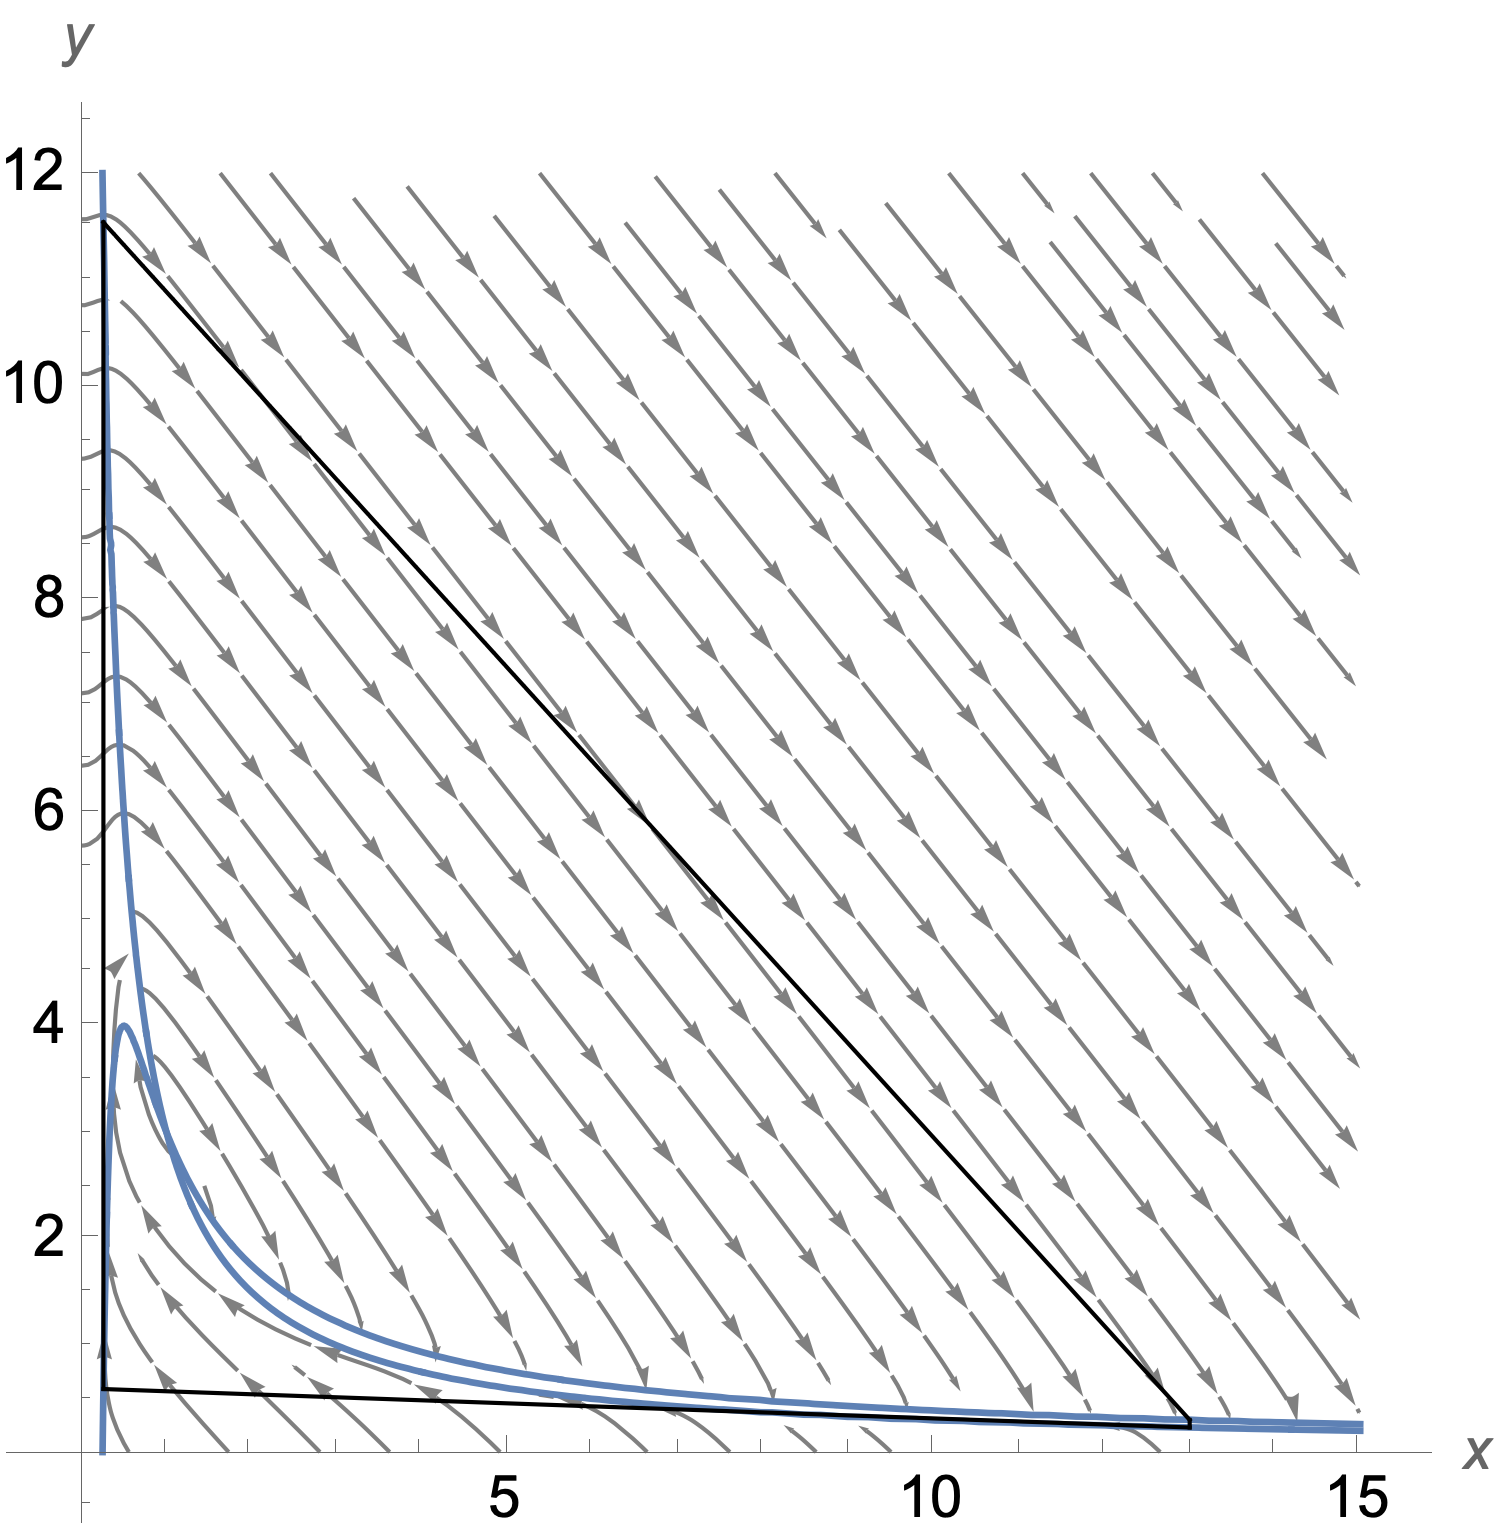
\includegraphics{img/PS08S23brusselatortrap.png}

This looks like it is a trapping region (with all vectors pointing inward).  On the upper right the flow looks steeper/inward.  On the bottom the flow also looks like the slopes work out for it to be inward.

\end{solution}
\item Do part (c) as written.
\begin{solution}
There is a Hopf bifurcation at $b_c = a+1$ (see part a).
\end{solution}
\item Assume that you have a trapping region where trajectories enter and do not leave for all values of $a,b>0$.  \emph{Note: this trapping region may include a fixed point.}
\begin{itemize}
\item Does the Poincar\'e-Bendixson theorem allow you to guarantee a closed orbit for $b>b_c$?  What about for $b<b_c$?
\item If there exists a closed orbit on only one side of the bifurcation, what kind of Hopf bifurcation would this likely be?
\item Provide a scenario where a different kind of Hopf bifurcation occurs at $b_c$ and a closed orbit would be present on both sides of $b_c$ \emph{This will involve a second bifurcation as well.  Identify them both.  Look at the squealing brake video for an example of this kind of scenario.} 
\end{itemize}
Note that the work you've done on this problem so far is not enough to distinguish between these two cases (the ones in the 2nd and 3rd bullet points).
\begin{solution}
\begin{itemize}
    \item When the fixed point is a repeller we can guarantee a closed orbit by creating a trapping region that excludes the repeller (and using a tiny circle about the repeller).  That allows us to create a new trapping region with no fixed points, so that we can use Poincaré-Bendixson.
    \item The limit cycle surrounds a repeller, so the bifurcation is likely supercritical.
    \item If the Hopf were subcritical and there were a saddle-node of limit cycles bifurcation, then there could be a closed orbit (specifically a stable limit cycle) present on both sides of $b_c$.
\end{itemize}
\end{solution}
\item Do part (e) as written.  You are asked for the period, rather than the frequency.
\begin{solution}
    The approximate period for the limit cycle is $2\pi/\omega$ where $\omega$ is the imaginary part of the eigenvalue at the bifurcation.  At $b_c = a + 1$ we have $\Delta = a = i\omega(-i\omega)=\omega^2$ so the period is approximately $2\pi/\sqrt{a}$.

    I will plot to check this:
    
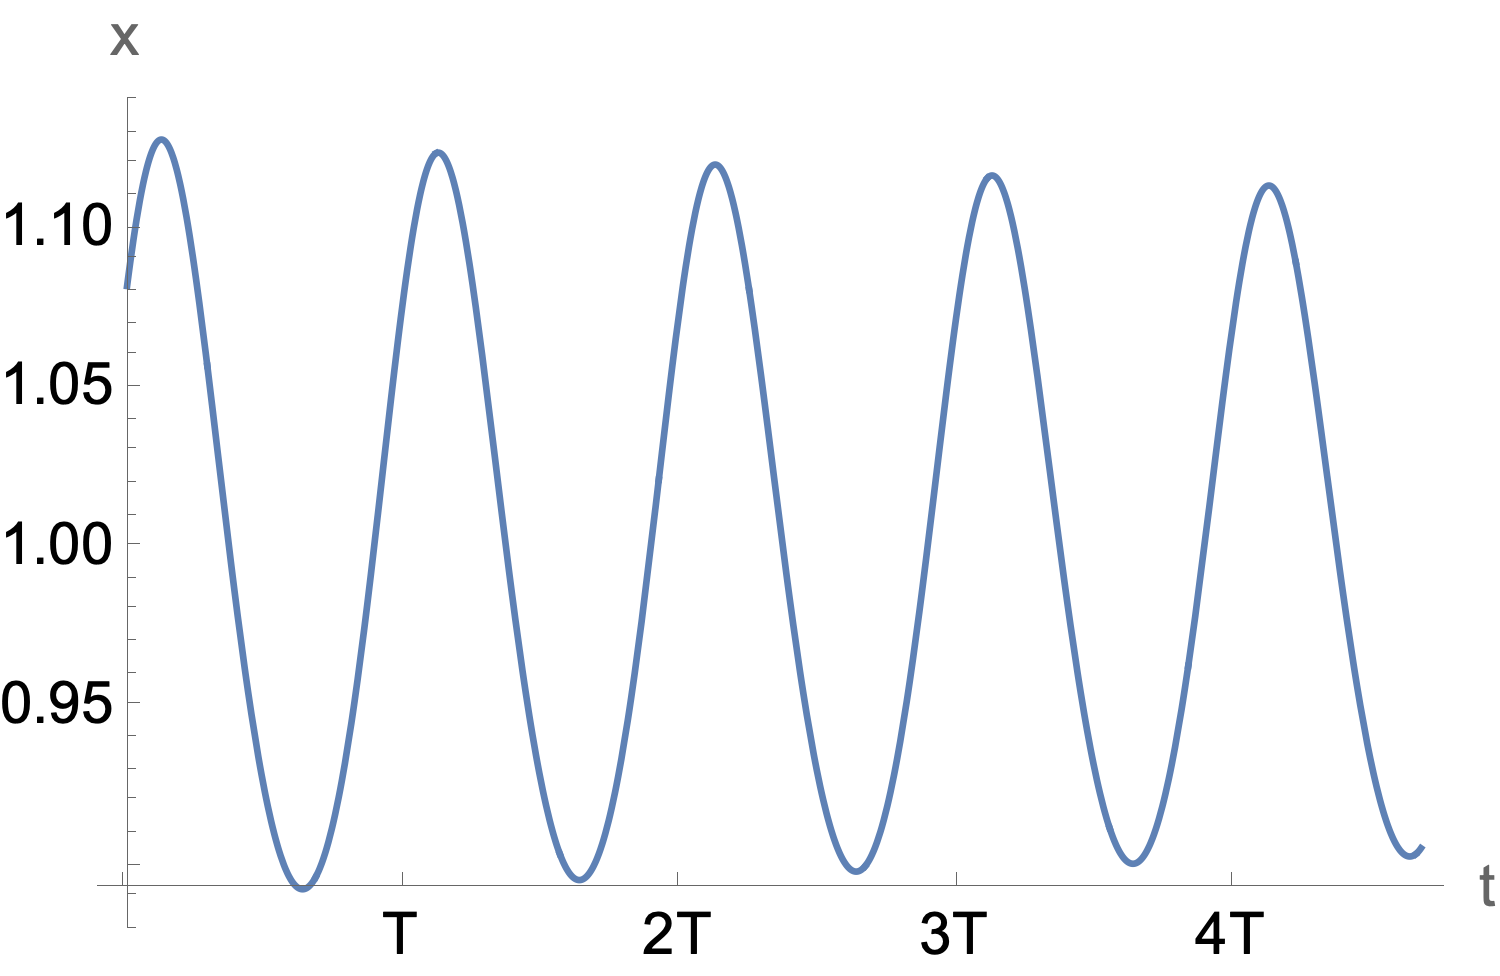
\includegraphics{img/PS08periodic.png}

$T = 2\pi/\sqrt{a}$, and that does look like it is approximately the period (I set $a = 1.5$ and $b = a+ 1$).
    
\end{solution}
\item Choosing two parameter sets, one set on either side of the bifurcation, use Mathematica/Python to add a trajectory to a phase portrait.

\begin{solution}

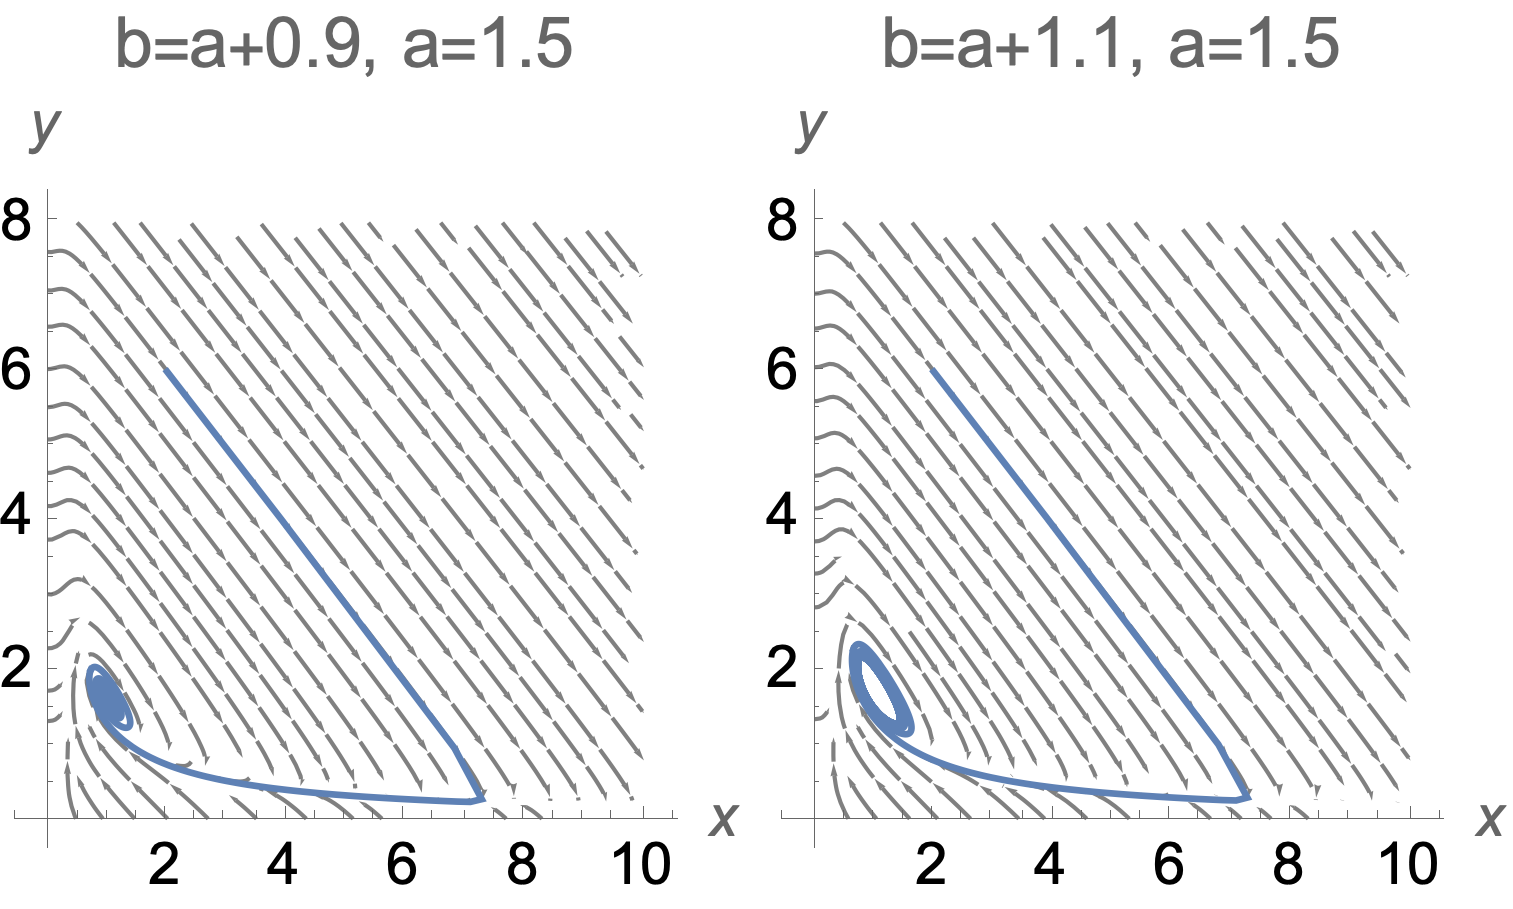
\includegraphics{img/PS08S23brusselatorphase.png}

\end{solution}


\end{parts}

\question Project proposal and project log.
\begin{parts}
    \item (proposal part 1) As a team, select three papers (book chapters are also fine).  At least one of the papers should be from the list I've provided.  At least one paper or book chapter should be found by your group.  The third can be from the list or elsewhere.  To submit the list of papers, have one member of your group email me with the other members of the group CCd.
    \item (proposal part 2) As part of your individual problem set work, write as little as a sentence and as much as a paragraph about each of the three papers/chapters/topics your group has selected.  This sentence/paragraph should be about what you personally find interesting about the paper.
    \item (project log) For the project log this week, there are two additional time categories in question 6 of the reflection questions.  Completing reflection questions 6f and 6g is all that you need to do for this log.
\end{parts}

\end{questions}

\vfill

\noindent\textbf{Project timeline} 

% \noindent\textbf{March 23} (Wednesday) project topic + team preferences submitted

% \noindent\textbf{March 25} (Wednesday) teams assigned (usually teams of 3, but 1 or 2 may be possible)

\noindent\textbf{March 29} (Wednesday) project proposal: this has been extended to March 31. 

\noindent\textbf{Weekly on Fridays in April} Individual project work log due: this is the core individual deliverable of the project work.

\noindent\textbf{April 19} (Wednesday) team progress report slides due

\noindent\textbf{April 21/24/26} (Friday/Monday/Wednesday) team progress report presentations

\noindent\textbf{May 10, 9am} (Wednesday) team final presentation slides due

\noindent\textbf{May 10, 2pm-5pm} (Wednesday) team final presentations; final individual log due

\end{document}
